\begin{enumerate}
    \item Order Products by Average Rating
    \item Most Reviewed Products
    \item Average Helpful Votes per Reviewer
    \item Number of Reviews with Images and positive Verfied Status
    \item Average Review Length
    \item Temporal Distribution of Reviews
    \item Distribution of Overall Ratings
    \item Number of Reviews by Verified Status and Rating
    \item Average Number of Votes for Verified vs. Non-Verified Reviews
    \item Average and Highest Rating per Format Style
\end{enumerate}

\subsection{Order Products by Average Rating}
The most straightforward query that can be performed is to order the products by their average rating, in order to understand which are the most appreciated ones. \\
\begin{lstlisting}[language=Java]
db.reviews.aggregate([
  { $group: { _id: "$asin", avg_rating: { $avg: "$overall" } } },
  { $sort: { avg_rating: -1 } }
]);
\end{lstlisting}
Results:
\begin{figure}[H]
  \centering
  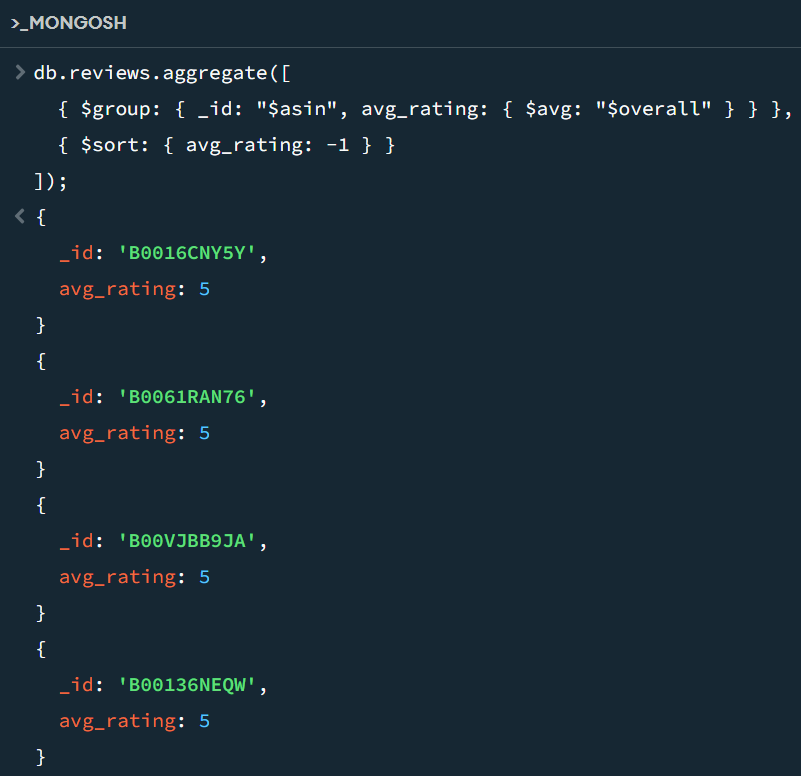
\includegraphics[scale=1]{Images/q1_result.png}
  \caption{Query 1 (partial) results}
  \label{fig:q1_result}
\end{figure}
As we can see from Figure \ref{fig:q1_result}, there are many products sharing the highest value for average rating, meaning that all the reviews that involve those products have the highest possible value, which is 5.\\

\subsection{Most Reviewed Products}
Another interesting query is to find the most reviewed products, in order to understand which are the most popular ones. \\
\begin{lstlisting}[language=Java]
db.reviews.aggregate([
  { $group: { _id: "$asin", count: { $sum: 1 } } },
  { $sort: { count: -1 } }
]);
\end{lstlisting}
Results:
\begin{figure}[H]
  \centering
  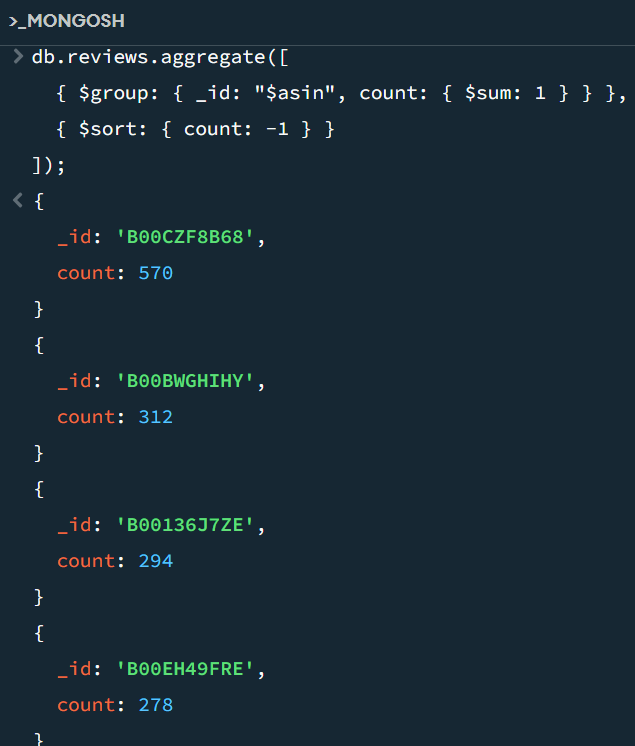
\includegraphics[scale=1]{Images/q2_result.png}
  \caption{Query 2 (partial) results}
  \label{fig:q2_result}
\end{figure}

\subsection{Average Helpful Votes per Reviewer}
We can write a query to find the average number of helpful votes per reviewer, in order to understand which are the most appreciated ones. \\
\begin{lstlisting}[language=Java]
db.reviews.aggregate([
  { $group: { _id: "$reviewerID", 
    avg_votes: { $avg: {$ifNull:[{$toInt: "$vote"}, 0]} } } },
  { $sort: { avg_votes: -1 } }
]);
\end{lstlisting}
In this case we decided to use the \texttt{\$ifNull} operator to handle the case in which the \texttt{vote} field is missing: in practice, we filled the missing values in this field by putting them equal to 0. \\
Results:
\begin{figure}[H]
  \centering
  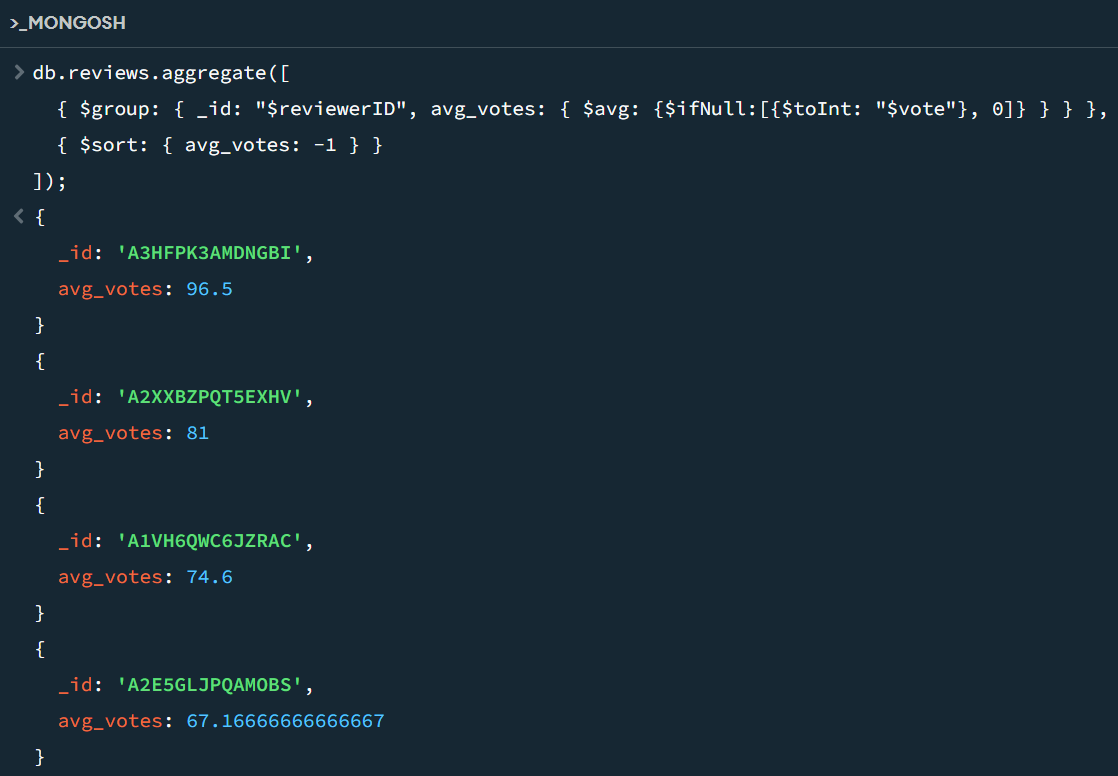
\includegraphics[scale=1]{Images/q3_result.png}
  \caption{Query 3 (partial) results}
  \label{fig:q3_result}
\end{figure}